\clearpage
\begin{column}{ミニ研究}

\textbf{Braessのパラドックスの検討 〜松山市のPT調査をもとに〜  }
{\small 冨矢航大}

\subsubsection*{Braessのパラドックス}
\label{sec:traffic-seeds}

都市の交通渋滞を解消するためには、新道の建設や車線拡幅が不可欠であると考えられがちです。しかし、利用者が自身の利益を最大化しようと経路を選択する「利用者均衡配分」の理論下では、特定の道が存在することで、かえって全体の効率が下がる「Braessのパラドックス」が生じることがあります。
ミニ研究として、松山市中心部のネットワークデータと、2007年のPT調査データを用いて、この現象を検証しました。混雑時間帯である朝8時台のトリップを対象に、全2,140本のリンクを一本ずつ仮想的に「消去」し、総旅行時間の変化を網羅的に計算しました。
その結果、全リンクの約40％に相当する854本において、その道を消去したほうが都市全体の総旅行時間を短縮できるという結果が得られました。その多くは微差に留まるものの、一本消去するだけで総旅行時間が1時間近く短縮されるリンクも確認されました。

\begin{center}
  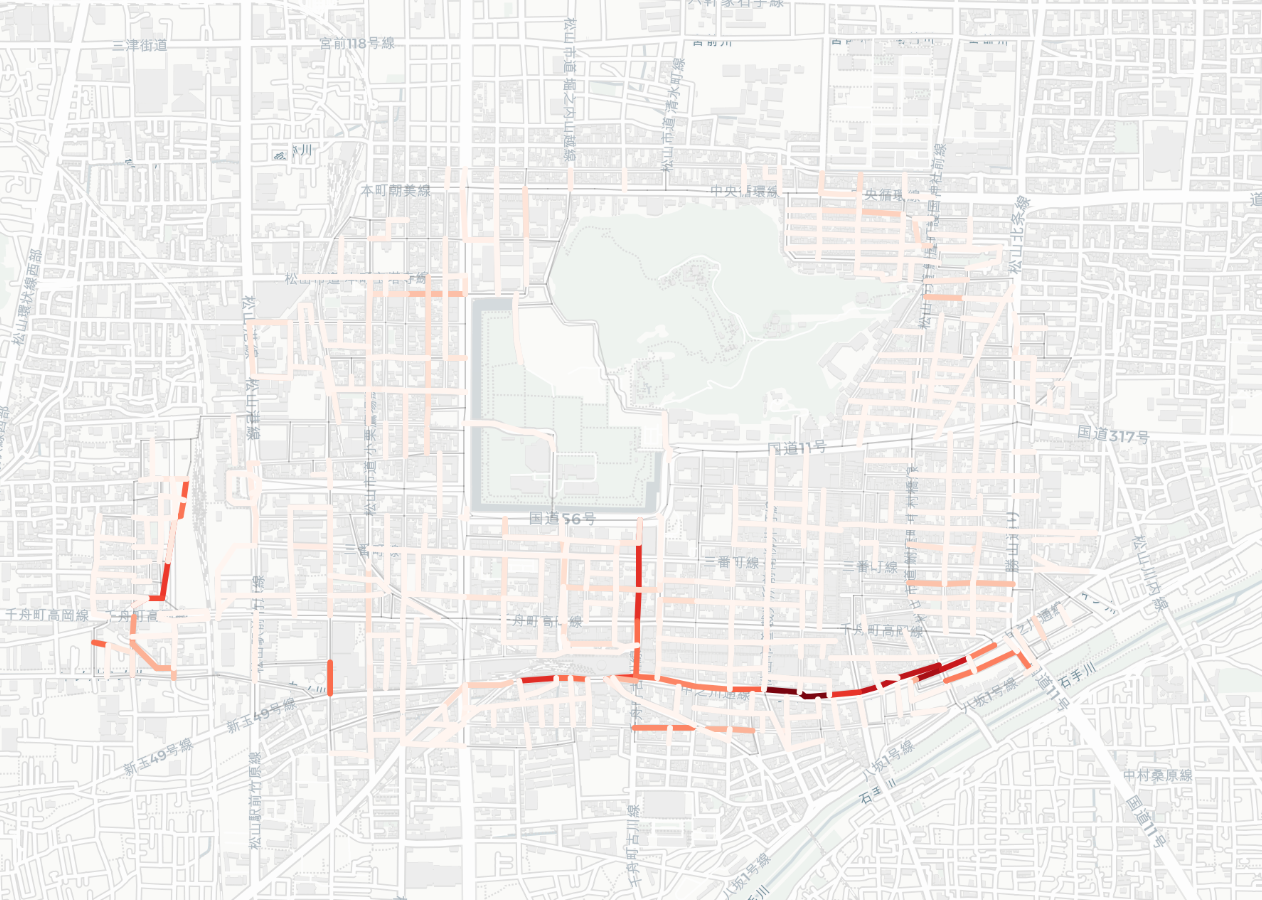
\includegraphics[width=\linewidth]{assets/assignment/pictureA.png}
  \captionof{計算結果を地図上に示したものです。図の色のついた道が消すことによって総旅行時間を減少させる道で、色が濃いほど減少効果が大きいことを示しています。}
  \label{fig:pictureA}
\end{center}


\subsubsection*{「中ノ川通り」閉鎖実験：なぜ主要幹線が渋滞を招くのか}

具体例として、松山市の主要幹線道路である「中ノ川通り」の東行き車線（松山市駅から離れる方向）に注目します。この道は片側3車線で交通量も多い区間ですが、シミュレーション上で図の青色の矢印付近のリンクを閉鎖したところ、全体の総旅行時間が約32分も短縮されるという結果が出ました。
交通の変化としては、中ノ川通りを閉鎖することで、それまで特定区間に集中していた交通が南北の隣接道路へと分散されます。
一見すると迂回によるロスが増えるように思えますが、閉鎖前、中ノ川通りの松山市駅付近（下図でむらさき色で囲った部分、閉鎖した区間よりも西側）において交通量が過剰であったために、この区間での時間ロスが大きくなっていました。
中ノ川通りの閉鎖によりこのむらさき色で囲った混雑区間の交通量が減少し、その減少効果は迂回による増加分を上回ったためにこのような結果が得られたと解釈しました。

\begin{center}
  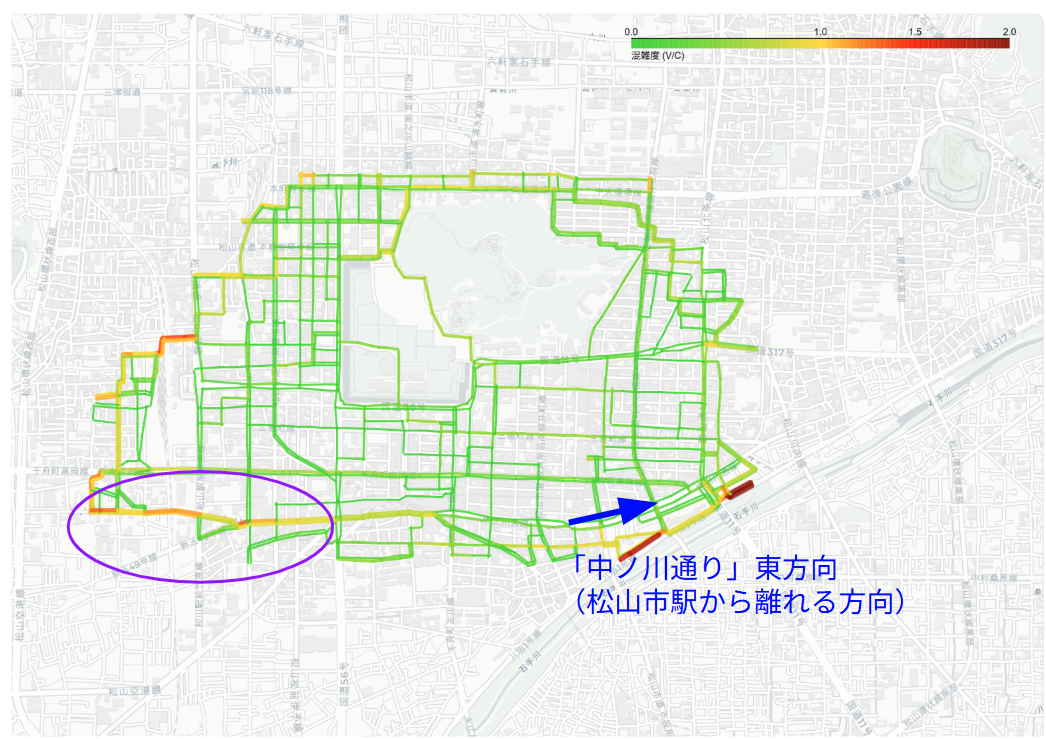
\includegraphics[width=\linewidth]{assets/assignment/pictureB.png}
  \captionof{各リンクの混雑度を図示したものです。オレンジ色や赤色のリンクが混雑していることを示しています。}
  \label{fig:pictureB}
\end{center}

\subsubsection*{JR松山駅高架化がもたらす効果}

現在進められているJR松山駅の高架化に合わせ、JR駅の下を通り抜ける道路が新設される計画となっています。
本検証では、実際に計画されているのと同じ駅を東西に貫く仮想道路（片側2車線、延長286m）を新設し、その影響を計測しました。その結果、都市全体の総旅行時間は18.89時間も減少するという結果が得られました。
新設道路により、既存の周辺道路の交通量は大きく変化します。シミュレーション上では、東行きで1249台、西行きで532台もの交通量が新設区間へと転換されました。
注目すべきは、これまで渋滞が激しかった特定区間の交通負荷を、新設リンクが「バイパス」として効率よく引き受けている（地図を拡大しているため分かりづらいですが、先ほどの図でむらさき色で囲ったリンクの交通量が大幅に減っている）点です。

\begin{center}
  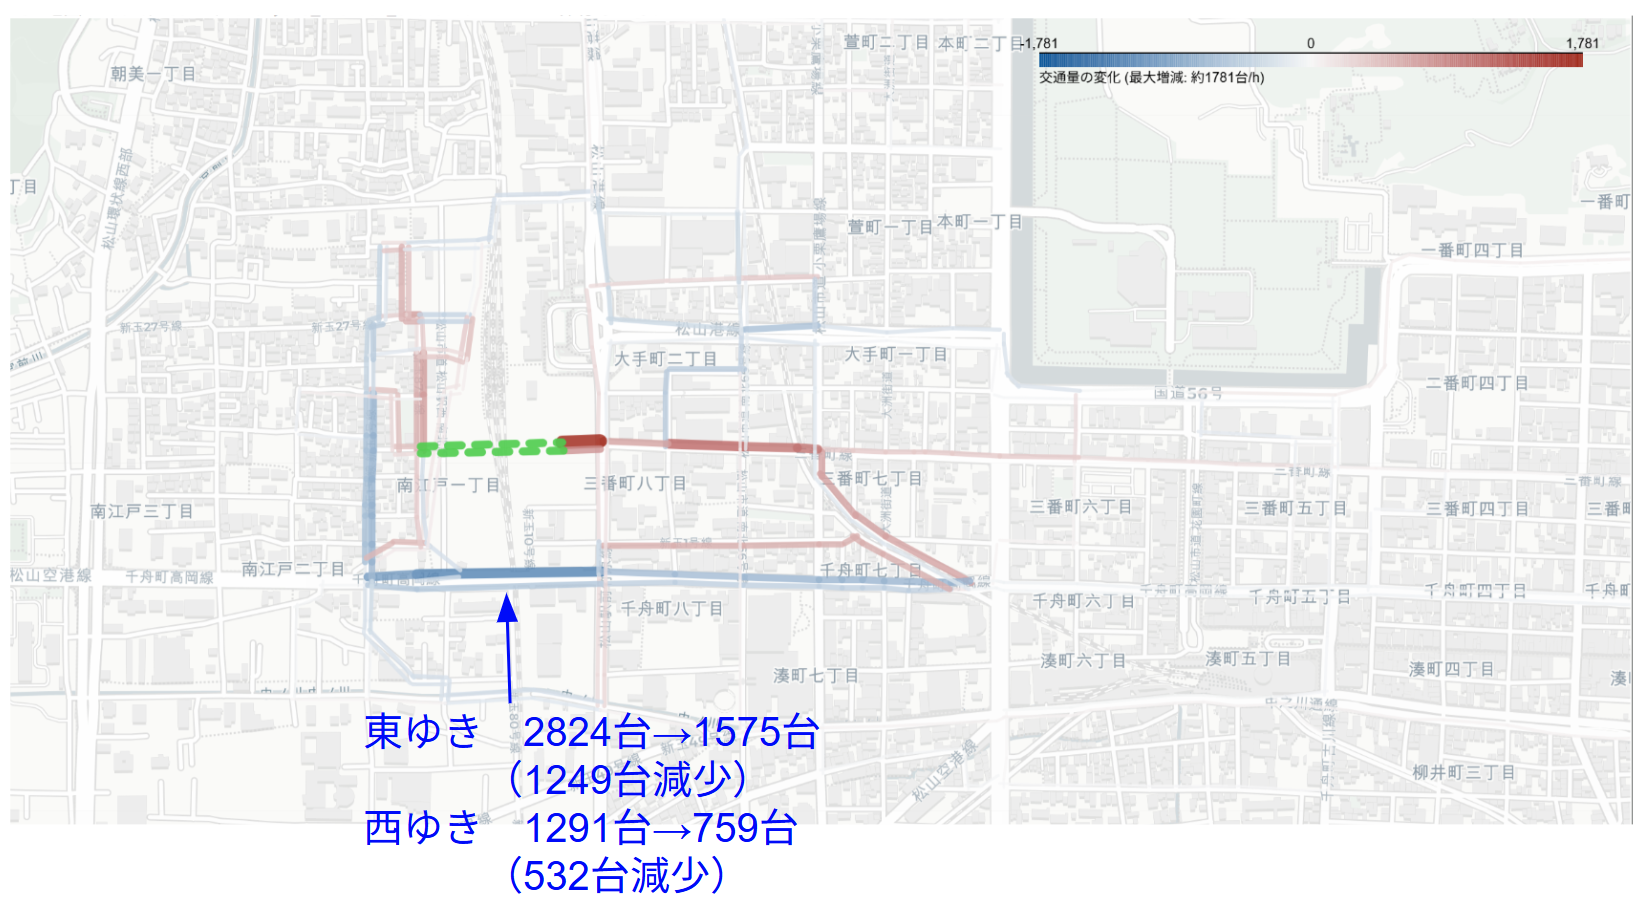
\includegraphics[width=\linewidth]{assets/assignment/pictureC.png}
  \captionof{黄緑色の点線が今回の検証で新設したリンク。この地図ではリンク新設の前後での交通量の増減を示しており、赤が増加・青が減少を示しています。}
  \label{fig:pictureC}
\end{center}

\subsubsection*{混雑緩和のメカニズム：下に凸の増加関数を攻略する}
なぜ、特定の地点への交通集中を緩和することが、これほどまでに大きな効果を生むのでしょうか。その鍵は、交通工学で用いられるリンクパフォーマンス関数（BPR関数）の性質にあります。
今回の計算に用いたリンクパフォーマンス関数は、本テキストでも既出の以下の式です。
\begin{equation}
  t_a(x_a) = t_{a0}\left\{1 + 0.15\left(\frac{x_a}{C_a}\right)^4\right\}
\end{equation}

これは交通量が増加するにつれ、旅行時間が急激に立ち上がる「下に凸の増加関数」です。つまり、渋滞ポイントで交通量を1台減らすことで得られる時間短縮効果が、空いている道路での1台の削減効果よりも圧倒的に大きくなります。
中ノ川通りの閉鎖による交通分散も、JR松山駅の新設道路によるバイパス効果も、本質的には「極端に混雑しているリンクの負荷を減らす」という点で共通しています。都市全体の旅行時間を最小化するためには、ボトルネックへの流入をいかに制御するかがポイントとなります。
　
\subsubsection*{結びに}
今回の検証は、松山市という実在の都市構造をモデル化することで、理論上のパラドックスが現実の都市計画においても十分起こり得ることを示唆しました。
道路を「消す」ことでも「加える」ことでも交通の流れを改善できる（逆に言えば悪化させる可能性もある）ということは、データに基づいたシミュレーションによる都市計画を進めることの重要さを示しています。

\end{column}
\clearpage

